\documentclass[a4paper,12pt]{book}
\usepackage{graphicx}
\title{Database System Concepts}
\author{Most.Jannat-ul-ferdoush}
\begin{document}
	\maketitle
	\newpage
	
	\chapter{Feasibility Study}
	\section{INTRODUCTION}
	A feasibility study in software engineering is a rigorous evaluation of the profitability and viability of a software development initiative. An IT consulting company with 10-year expertise, ScienceSoft helps businesses understand whether a new software project is worth their time and money.
	\\Feasibility Study Process : \\
	\begin{enumerate}
	\item	Information assessment
	\item Information collection
	\item Report writing
	\item General information
		\end{enumerate}
	The next step is to determine exactly candidade system needed.\\
	\section{Need of Feasibility Study in The Company:} 
	Feasibility study is so important stage of Software Project Management Process as after completion of feasibility study it gives a conclusion of whether to go ahead with proposed project as it is practically feasible or to stop proposed project here as it is not right/feasible to develop or to think/analyze about proposed project again.\\
	Along with this Feasibility study helps in identifying risk factors involved in developing and deploying system and planning for risk analysis also narrows the business alternatives and enhance success rate analyzing different parameters associated with proposed project development.
	\section{System Performance}
	Performance is an indicator of how well a software system or component meets its requirements for timeliness. Timeliness is measured in terms of response time or throughput. The response time is the time required to respond to a request. It may be the time required for a single transaction, or the end-to-end time for a user task. For example, we may require that an online system provide a result within one-half second after the user presses the "enter" key. For embedded systems, it is the time required to respond to events, or the number of events processed in a time interval. The throughput of a system is the number of requests that can be processed in some specified time interval. For example, a telephony switch may be required to process 100,000 calls per hour.
	
\begin{figure}[h]
	\centering
	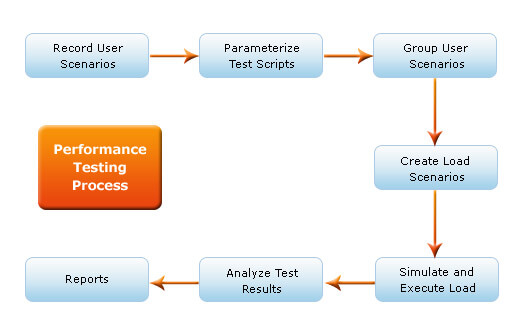
\includegraphics[width=0.7\linewidth]{Performance-Testing-Process}
	\caption{System performance diadram}
	\label{fig:performance-testing-process}
\end{figure}
\section{Statement of Constraints}
	Constraints are a factor that limit the solution of the problem.\\
	The three basic constraints, which are the synchronizing support effect disappearance constraint, the minimum oscillation frequency constraint of low frequency oscillations and the frequency stability constraint, consist of a triangle criterion to determine the reasonable size of the synchronous grids.\\
	It is the fact that there are only so many hours in a day to accomplish things. One that restricts, limits, or regulates.\\	
\begin{figure}[h]
	\centering
	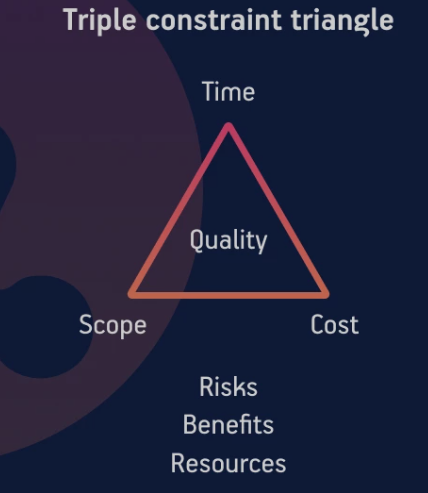
\includegraphics[width=0.6\linewidth]{7_1}
	\caption{constraints level diagram}
	\label{fig:71}
\end{figure}
\section{Identification of Specific System Objective}

\end{document}